\documentclass[a4paper,11pt]{article}
\usepackage[T1]{fontenc}
\usepackage[polish,english]{babel}
\usepackage[utf8]{inputenc}
\usepackage{lmodern}
\usepackage{graphicx}

\title{Sauron - projekt wstępny}
\author{Mateusz Forc, \\ Grzegorz Staniszewski, \\ Wiktor Franus, \\ Przemysław Kopański}

\begin{document}

\selectlanguage{polish}

\maketitle
\tableofcontents

\newpage
\section{Treść zadania}
W pierścieniu połączone są serwer i N czujników. Serwer jest stale aktywny. Czujniki periodycznie budzą się i wykonują pomiar. Każdy czujnik próbuje odebrać komunikat z pomiarami od jednego sąsiada, dodać do niego swój pomiar i wysłać drugiemu sąsiadowi. Czujniki oszczędzają energię, zatem należy minimalizować czas ich pracy i wolumin transmitowanych danych. Sieć ma tolerować pojedyncze uszkodzenie węzła lub połączenia. Należy zaprojektować i wykonać system komunikacji dla tej sieci. Przeanalizować wybór protokołu IPv4 i IPv6. Ponadto należy zaprojektować moduł do Wireshark umożliwiający wyświetlanie i analizę zdefiniowanych komunikatów.

\section{Założenia funkcjonalne}

\begin{enumerate}
  \item Serwer
  \begin{enumerate}
    \item inicjalizuje sieć czujników
    \item ustala tryb pomiaru wspólny dla wszystkich czujników
    \item uruchamia pomiar
    \item przechowuje informacje o czujnikach oraz wykonywanych pomiarach
    \item rozpoznaje miejsca awarii sieci i wypisuje komunikaty
    \item w przypadku awarii jednego czujnika przystosowuje sieć do poprawnego funkcjonowania
    \item w przypadku wykrycia więcej niż jednej awarii wyłącza system
  \end{enumerate}
  \item Czujnik
  \begin{enumerate}
    \item periodycznie budzi się i wykonuje pomiar
    \item próbuje odebrać komunikat z pomiarami od jednego sąsiada
    \item dodaje do odebranego komunikatu swój pomiar i wysyła go drugiemu sąsiadowi
  \end{enumerate}
  \item Aplikacja wspiera IPv4 i IPv6.
  \item Konfiguracja sieci pobierana jest z pliku.
\end{enumerate}

\section{Założenia niefukncjonalne}

\begin{enumerate}
  \item Serwer jest stale aktywny.
  \item Sieć ma tolerować pojedyncze uszkodzenie węzła lub połączenia.
  \item Minimalizacja czasu pracy czujników i ilości transmitowanych danych.
\end{enumerate}

\section{Przypadki użycia}\label{PU}

\subsection{Włączenie systemu}
Aktorzy: użytkownik\\
Scenariusz główny:
\begin{enumerate}
   \item Użytkownik wprowadza do pliku konfiguracyjnego adresy czujników i tryb pomiaru    
   \item Użytkownik uruchamia aplikację (serwer)
   \item Serwer inicjalizuje czujniki
   \item Serwer wypisuje komunikat o sukcesie
   \item Serwer rozpoczyna wykonywanie pomiarów przez czujniki
   \item Serwer wypisuje na ekran pomiary otrzymane z czujników
\end{enumerate}
Scenariusz alternatywny 1: (Jeden czujnik nie działa na etapie inicjalizacji)
\begin{enumerate}
   \item [1-3.] jak w scenariuszu głównym
   \item [4.] Serwer wypisuje ostrzeżenie z informacją o niedziałającym czujniku
   \item [5-6.] Jak w scenariuszu głównym
\end{enumerate}
Scenariusz alternatywny 2: (Więcej niż jeden czujnik nie działa na etapie inicjalizacji)
\begin{enumerate}
   \item [1-3.] jak w scenariuszu głównym
   \setcounter{enumi}{3}
   \item Serwer wypisuje komunikat o awarii systemu
   \item Serwer usypia działające czujniki
   \item Serwer kończy działanie jak w PU \ref{turnoff}
\end{enumerate}
Scenariusz alternatywny 3: (Jeden czujnik przestaje działać po etapie inicjalizacji)
\begin{enumerate}
   \item [1-5.] jak w scenariuszu głównym
   \setcounter{enumi}{5}
   \item Serwer wypisuje ostrzeżenie z informacją o niedziałającym czujniku
   \item Serwer wypisuje na ekran pomiary otrzymane z czujników
\end{enumerate}
Scenariusz alternatywny 4: (Więcej niż jeden czujnik przestaje działać po etapie inicjalizacji)
\begin{enumerate}
   \item [1-5.] jak w scenariuszu głównym
   \setcounter{enumi}{5}
   \item Serwer wypisuje komunikat o awarii systemu
   \item Serwer usypia działające czujniki
   \item Serwer kończy działanie jak w PU \ref{turnoff}
\end{enumerate}

\subsection{Wyłączenie systemu}\label{turnoff}
Scenariusz główny:
\begin{enumerate}
   \item Serwer usypia działające czujniki
   \item Serwer wypisuje komunikat o pomyślnym uśpieniu czujników i kończy działanie
\end{enumerate}
Scenariusz alternatywny 1: (Nie wszystkie czujniki zostały uśpione)
\begin{enumerate}
   \item Jak w scenariuszu głównym
   \item Serwer wypisuje informację o niepoprawnie uśpionych czujnikach i kończy działanie
\end{enumerate}

\subsection{Wyłączenie systemu przez użytkownika}
Scenariusz główny:
\begin{enumerate}
   \item Użytkownik zleca serwerowi zakończenie pracy
   \item Serwer kończy działanie jak w PU \ref{turnoff}
\end{enumerate}

\section{Wybranie środowisko sprzętowo-programowe i narzędziowe}

\begin{enumerate}
  \item System operacyjny: GNU Linux (dystrybucje: ArchLinux, Ubuntu)
  \item Języki programowanie: C, C++ (aplikacja), Lua (wtyczka do Wireshark)
  \item Biblioteki: API gniazd BSD, Boost
  \item Narzędzia pomocnicze: Git, Gerrit, Github, gdb, Wireshark
\end{enumerate}

\newpage
\section{Architektura rozwiązania}
Architektura rozwiązania jest połączeniem architektury pierścieniowej i klient-serwer. W sieci pierścieniowej połączone są ze sobą czujniki - dokonujące pomiaru, wraz z serwerem głównym - zbierającym wyniki oraz zestawiającym całą sieć do poprawnej transmisji. Dodatkowo, czujniki pełnią rolę serwera pośredniczącego; ze względu na budowę sieci muszą one odbierać i przekazywać wyniki pomiarów innych czujników oraz informacje organizacyjne sieci.

\begin{center}
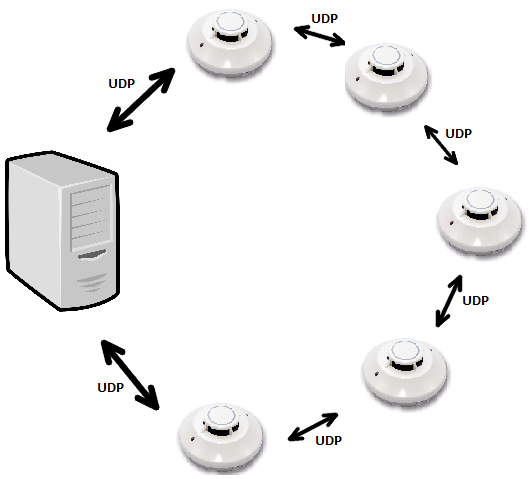
\includegraphics[scale=0.5]{architektura}
\end{center}

\subsection{Inicjalizacja}
Serwer trzyma listę adresów IP należących do pierścienia. Wyznacza nastepnie podziałkę w ich połowie - od tej pory komunikacja będzie odbywać się tylko w dwóch połowach pierścienia niezależnie zgodnie z zasadą dziel i zwyciężaj (oszczędzamy wolumin danych i ułatwiamy zarządzanie nimi w normalnym trybie pracy).
Do wyznaczonych połówek wysyłane są adresy określające połowy pierścienia wraz z kierunkiem przesyłania pomiarów. Serwer oczekuje na informację zwrotną z obu połówek świadczącą o braku błędów podczas inicjalizacji. Każdy czujnik po wysłaniu wiadomości oczekuje na odpowiedź, co umożliwia wykrycie pojedynczej awarii sieci.
\newpage
Czujnik pracuje w dwóch trybach naprzemiennie:
\begin{itemize}
\item w trybie aktywnym (okienko czasowe), w którym oczekuje na wynik od sąsiada, dokonuje pomiaru, przesyła jego wynik do drugiego sąsiada, odbiera i przesyła pozostałe komunikaty,
\item w trybie nieaktywnym, w którym nasłuchuje tylko na wybrane komunikaty
\end{itemize}
Inicjalizacja czujników następuje w pojedyńczym okienku czasowym. Pierwszy pomiar jest wykonany w kolejnym okienku czasowym. 

\subsubsection{AWARIA 1: węzeł nie odpowiada podczas inicjalizacji}
Węzeł, który nie otrzymał odpowiedzi zwrotnej od sąsiada podczas inicjalizacji, zwraca w przeciwną stronę informację o błędzie zawierającą adres IP węzła, który nie odpowiedział. Informacja z błędem trafia ostatecznie do serwera. Serwer rozpoczyna inicjalizację czujników od początku, dostosowując listy adresów czujników w obu połówkach pierścienia, w sposób umożliwiający poprawną komunikację z jednym niedziałającym czujnikiem. 
%dodac rysunek jak zostaly wezly podzielone, ktory to jest wezel graniczny, i w ktorym kierunku nastepuje przesylanie pomiarow

\subsection{Tryb pomiaru}
Pomiary startują automatycznie w okienku czasowym następującym po inicjalizacji (równocześnie we wszystkich węzłach). Transport wyników pomiarów rozpoczyna się w węzłach granicznych i postępuje w kierunku serwera. Kolejne węzły oczekują na wyniki od poprzedników, dokładają do zbioru własny pomiar oraz przekazują je następnikom. Po każdej wysłanej wiadomości węzeł oczekuje na jej potwierdzenie, brak potwierdzenia oznacza awarię węzła.

\subsubsection{AWARIA 2: węzeł nie odpowiada podczas zbierania wyników pomiarów}
Węzeł, który nie otrzymał potwierdzenia od adresata wiadomości zawierającej zbiór pomiarów, wysyła w przeciwnym kierunku tą samą wiadomość dodając do niej informację o adresie wadliwego węzła. Czujnik znajdujący się po drugiej stronie wadliwego węzła, nie otrzymawszy w dopuszczalnym czasie od poprzednika żadnej wiadomości, przesyła do kolejnego węzła swój pomiar dołączając do wiadomości adres wadliwego węzła. Serwer z dwóch stron otrzymuje informację o pomiarach i wadliwym czujniku. Jeśli adresy otrzymane z dwóch stron są różne to zaszła awaria więcej niż jednego czujnika. Serwer przystępuje wtedy do wyłączania czujników. Jeśli serwer otrzymał od obu sąsiadów ten sam adres wadliwego czujnika, oznacza to, że tylko jeden węzeł doznał awarii. W tym przypadku serwer dokonuje ponownej inicjalizacji sieci dostosowując odpowiednio listę adresów IP w obu połówkach pierścienia.

%goodbye + errors

\section{Sposób testowania}
\begin{itemize}
  \item Testy jednostkowe dla wszystkich modułów napisane w Boost Test Unit
  \item Testy integracyjne
  \item Możliwość uruchomienia wszystkich rodzajów testów za pomocą jednego polecenia
\end{itemize}

\section{Sposób demonstracji rezultatów}
Działanie systemu zostanie zaprezentowane przy pomocy kilku komputerów podłączonych do jednej podsieci za pomoca routera. Jeden z komputerów pełnić będzie rolę serwera, zaś pozostałe - czujników. Zademonstrowane prowadzącemu zostaną scenariusze opisane w punkcie \ref{PU}.

\section{Podział prac w zespole}
Prace nad projektem wykorzystują jedną z metod programowania zwinnego, tj. pair programming - każde zadanie przydzielane jest parze. Pary oceniają nawzajem stworzony przez siebie kod przy uzyciu narzędzia do rewizji kodu Gerrit. Istnieją zadania, które wykonuje cały zespół lub sam lider. \\
Przydział zadań:
\begin{enumerate}
\item Sprint 1 - dokumentacja wstępna i repozytorium
\begin{itemize}
\item Stworzenie dokumentacji wstępnej - cały zespół
\item Utworzenie repozytorium na Github - Mateusz Forc (lider)
\item Integracja repozytorium z Gerrit - Mateusz Forc (lider)
\item Założenie kont dla programistów oraz prowadzącego - Mateusz Forc (lider)
\item Stworzenie instrukcji korzystania z Gerrit oraz ustalenie stylu kodowania - Mateusz Forc (lider)
\end{itemize}
\item Sprint 2 - implementacja podstawowych funkcjonalności
\begin{itemize}
\item Projekt komunikatów - cały zespół
\item Wtyczka do Wireshark - Grzegorz Staniszewski, Przemysław Kopański
\item Wrapper API gniazd BSD - Mateusz Forc (lider), Wiktor Franus
\item Testy jednostkowe wrappera w zakresie podstawowym - Mateusz Forc (lider), Wiktor Franus
\item Projekt i implementacja modułu serwera wraz z podstawowymi funkcjonalnościami - Mateusz Forc (lider), Wiktor Franus
\item Projekt i implementacja modułu klienta (czujnika) wraz z podstawowymi funkcjonalnościami - Grzegorz Staniszewski, Przemysław Kopański
\item Testy jednostkowe modułów serwera w zakresie podstawowym - Mateusz Forc (lider), Wiktor Franus
\item Testy jednostkowe modułów klienta w zakresie podstawowym - Grzegorz Staniszewski, Przemysław Kopański
\item Podstawowe testy integracyjne aplikacji - Grzegorz Staniszewski, Przemysław Kopański
\item Wczytywanie konfiguracji sieci z pliku - Grzegorz Staniszewski, Przemysław Kopański
\item Aktualizacja zadań w sprincie 2 i 3 w ramach dokumentacji - Mateusz Forc (lider)
\end{itemize}
\item Sprint 3 - kompletna implementacja wraz ze wszystkimi testami
\begin{itemize}
\item Uzupełnienie testów jednostkowych wrappera - Mateusz Forc (lider), Wiktor Franus
\item Implementacja pozostałych funkcjonalności modułu serwera - Mateusz Forc (lider), Wiktor Franus
\item Implementacja pozostałych funkcjonalności modułu klienta - Grzegorz Staniszewski, Przemysław Kopański
\item Pozostałe testy modułu serwera - Mateusz Forc (lider), Wiktor Franus
\item Pozostałe testy modułu klienta - Grzegorz Staniszewski, Przemysław Kopański
\item Uodpornienie programu na niepożądane parametry od użytkownika - Grzegorz Staniszewski, Przemysław Kopański
\end{itemize}
\end{enumerate}
Ze względu na dynamiczny charakter pracy kolejność i zakres zadań oraz podział na pary i sprinty może ulec zmianie. 

\section{Harmonogram prac}
Sprint 2 - od 19.04 do 12.05 \\
Sprint 3 - od 12.05 do 28.05 \\

\section{Adres projektu}
Repozytorium kodu dostępne jest w serwisie Github pod adresem:
\begin{center}https://github.com/formateu/sauron \end{center}
Dostęp do repozytorium jest ograniczony do kont posiadających uprawnienia do jego odczytu. Dane konta prowadzącego są dostarczone razem z niniejszą dokumentacją wstępną.
\end{document}
\grid
